\section{Site de liaison d'allèle spécifique}
Dans cette partie sera présenté une manière plus affiné de détecté les sites de liaisons. 
\subsection{Définition}
Pour commencer un transcription, une protéïne est nécessaire. Celle-ci doit se fixer sur l'hélice. Une liaison d'allèle spécifique est ce même phénomène mais avec une protéine qui se liera d'avantages sur les allèles récessives.

\subsection{allèles préférées}

Une des premières observations faites est que sur les individus hétérozygotes (ayant deux allèles différentes) on remarque que certaines allèlles créent plus de sites de connections que une autre, alors que il était possible de s'attendre à une distribution equi-probable. 
\newline
\newline
Mais comme les allèles fortes s'expriment plus que les allèles récessives celà peut être dû à plusieurs raisons mais la plus commune est que, par selection naturelle, un gène subira une mutation, et aura un nombre supérieur de site de transcriptions que le précédent et ainsi pourra se transmettre plus facilement de génération en génération. De ce fait l'étude à de meilleurs chances de résultats si il est éffectué sur des gènes forts.
\begin{figure}{l}{}
\centering
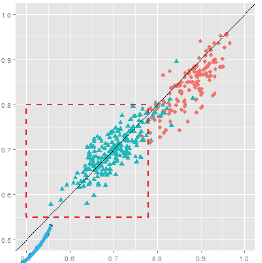
\includegraphics{grapheBestAllele}
\newline
\color{blue}
$\triangle$
\color{black} Allèles récessives
\\
\color{red}
$\Box$
\color{black} Allèles fortes
\caption{Allèle score}
\end{figure}


Pour trouver les places de liaisons de transcription, une unité a été crée: \textbf{PWM}: La matrice de position de poids.\\
Il s'agit d'une matrice où sont marquées les probabilités de chaque nucléotide d'apparaitre dans le site de liaison pour la transcription, ainsi que sa position.
\newline
\newline
Ceci a une importance particulière car grâce à ces matrices, il a été possible de remarquer que les liaisons ce faisaient plus sur les allèles récessives que les autres.
\newline
Mais ces travaux sont ralentis par le fait qu'il peut exister de multiples facteurs qui modifient le taux de transcription d'un site comme les mutations, l'hérédité et l'epigenetique.
\subsection{Recheche de site de liaison pour la transcription pour les lymphomes}

C'est ici que la présentation recoupe avec les travaux du Dr. Wasserman.
\newline
En effet, grâce aux outils présentés précédemment, beaucoup de données ont été recueillis, notamment des échantillons d'ADN, d'ARN de malades atteints de lymphomes.
\newline
\newline
Ensuite certaines zones du génomes ont été ciblés, et une des premières remarques est que les sites de transcriptions ont eu des taux de mutations plus élevé comparés aux séquences saines.
\newline
\newline
La mort des cellules, à un rôle dans ce fonctionnement. En effet, la mort des cellules est régulé d'une manière naturel et saine mais si cette régulation est perturbée celà peut causer des problèmes, dans le cas d'une diminution et dans le cas d'une augmentation un lymphome, par exemple. Une augmentation des cellules (ou plutôt une non décroissance normale du nombre de cellules) augmentent le nombre de site de liaison augmente. 


